The basic relationship types are listed in Table \ref{fig:table:rels}.

yano $\to$ grandmother $=$ yano $\to$ mother $\to$ mother

yano $\to$ brother $=$ yano $\to$ mother $\to$ son or yano $\to$ father $\to$ son  
      

\begin{table}[!h]
  \centering
  \subfloat[][]{\begin{tabular}{l}
    \toprule
    $yano \to mother$ \\
    \midrule
    $yano \to wife$ \\
    \midrule
    $yano \to daughter$ \\
    \midrule
    $yano \to girlfriend$ \\
        \midrule
    $yano \to friend$ \\
      \midrule
    $yano \to neighbour$ \\
      \midrule
    $yano \to classmate$ \\
     \midrule
    $yano \to colleague$ \\
    \bottomrule
  \end{tabular}}
  \qquad
  \subfloat[][]{\begin{tabular}{l}
    \toprule
    $yano \to father$ \\
    \midrule
    $yano \to husband$ \\
    \midrule
    $yano \to son$\\
    \midrule
    $yano \to boyfriend$ \\
      \midrule
    $yano \to acquaintance$ \\
      \midrule
    $yano \to housemate$ \\
    \midrule
    $yano \to teammate$ \\
    \midrule
    $yano \to ex$ \\
    \bottomrule
  \end{tabular}}
  \caption{The basic relationship types.}
  \label{fig:table:rels}
\end{table}

\begin{figure}[!h]
\begin{center}
\small
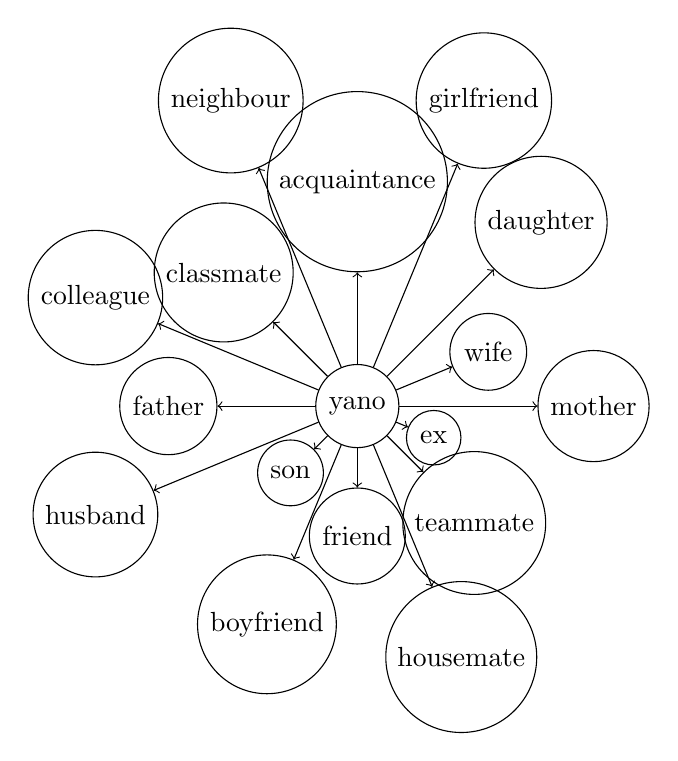
\begin{tikzpicture}[scale=3]
\tikzstyle{every node}=[draw,shape=circle];
\draw (0:0cm) node       (y0) {yano};
\draw (0:1cm) node       (y1) {mother};
\draw (22.5:0.6cm) node  (y2) {wife};
\draw (45:1.1cm) node      (y3) {daughter};
\draw (67.5:1.4cm) node  (y4) {girlfriend};
\draw (90:0.95cm) node      (y5) {acquaintance};
\draw (112.5:1.4cm) node (y6) {neighbour};
\draw (135:0.8cm) node     (y7) {classmate};
\draw (157.5:1.2cm) node (y8) {colleague};
\draw (180:0.8cm) node     (y9) {father};
\draw (202.5:1.2cm) node (y10) {husband};
\draw (225:0.4cm) node     (y11) {son};
\draw (247.5:1cm) node   (y12) {boyfriend};
\draw (270:0.55cm) node     (y13) {friend};
\draw (292.5:1.15cm) node   (y14) {housemate};
\draw (315:0.7cm) node     (y15) {teammate};
\draw (337.5:0.35cm) node (y16) {ex};

\tikzset{every node/.style={fill=white}} 
\draw (y0) edge [->] (y1);
\draw (y0) edge [->] (y2);
\draw (y0) edge [->] (y3);
\draw (y0) edge [->] (y4);
\draw (y0) edge [->] (y5);
\draw (y0) edge [->] (y6);
\draw (y0) edge [->] (y7);
\draw (y0) edge [->] (y8);
\draw (y0) edge [->] (y9);
\draw (y0) edge [->] (y10);
\draw (y0) edge [->] (y11);
\draw (y0) edge [->] (y12);
\draw (y0) edge [->] (y13);
\draw (y0) edge [->] (y14);
\draw (y0) edge [->] (y15);
\draw (y0) edge [->] (y16);
 \end{tikzpicture}
 \caption{A graph representation of thebasic relationship types.}
  \label{fig:img:grapgrep}
  \end{center}
\end{figure}
